\documentclass[11pt]{article}

%%% Page Setup
\usepackage[nohead,
            left=0.75in,right=0.75in,top=1.0in,
            footskip=0.5in,bottom=1.0in,     % Room for page numbers
            columnsep=0.33in
            ]{geometry}
\usepackage{graphicx}
\usepackage{listings}
\usepackage{minted}
\usepackage{subfig}
\usepackage{hyperref}
\usepackage{natbib}
\newcommand{\ttt}[1]{\texttt{#1}}
\usepackage{mathtools}
\DeclarePairedDelimiter{\ceil}{\lceil}{\rceil}
\usepackage{amsmath}
\newcommand*\textfrac[2]{
  \frac{\text{#1}}{\text{#2}}
}
\usepackage{caption}
\newcommand{\Km}{\mathbf{K}}

\title{15-418\\
       Final Project: Lock-Free Skip List}
\author{Mckenna Brown (mckennab); Grace An (gean)}
\begin{document}
\maketitle

\section{Summary}
We implemented three versions of skip lists using C/C++ and manual memory management: a coarse-grained locking skip list, a concurrent fine-grained locking skip list, and a concurrent lock-free skip list. We analyzed and measured their performance on different workloads on the GHC and PSC machines. Through performance benchmarking on the PSC machines, we confirmed Herlihy et al's claim that their fine-grained locking skip list had approximate performance to the lock-free skip list under all scenarios except for cases of high contention. We also found that by using 128 threads, on some workloads, we could perform 40x the number of operations in the same amount of time on the fine-grained and lock-free skip list as compared to the coarse-grained locking list (which forces all operations to be done sequentially). 
\section{Background}
\subsection{Skip List Motivation}
Skip lists tackle the problem of large scale concurrent data structures that offer efficient searching, insertion, and removal. Linked lists support the ability for different threads to expand the list in different areas without contention/dependencies. However, they are slow to search, even if sorted, as a given index cannot be indexed in O(1) time like is necessary for binary search. A popular choice for concurrent \ttt{key : value} storage is binary search trees that use randomness, but they are very complex to implement and extremely difficult to ensure correctness.

The skip list offers a lighter weight alternative that is flexible enough to handle different distributions (and relatively robust against non-uniform workloads). The key idea is similar to driving from one city to another that is far away: driving just among residential roads would be very slow and you'd have to read a lot of street signs. It requires far less navigational computation to go to a highway, and only get off the highway when your destination is nearing.

A skip list uses a similar idea by maintaining a hierarchy of different linked lists of elements ordered by keys. At the lowest level 0, which is analogous to residential roads, we have a simple skip list which is ordered by keys and contains pointers to arbitrarily typed values.

The higher levels leave 'gaps' (or 'skips') in their linked lists that allow for quick traversal over keys. Say you're searching for a node with key \ttt{k}. If you are at a level \ttt{i} and the current node you're at has key \ttt{a}, with the next key being \ttt{b}, such that \ttt{a < k < b}, then the key is either not in the list or is in a more detailed lower level list. We can then traverse downwards to search through a lower-level skip list. In this fashion, we use the higher levels of the linked list to skip over as many keys as possible to decrease the number of nodes that need to be traversed to find a given key. 

\begin{figure}[h!]
\begin{center}
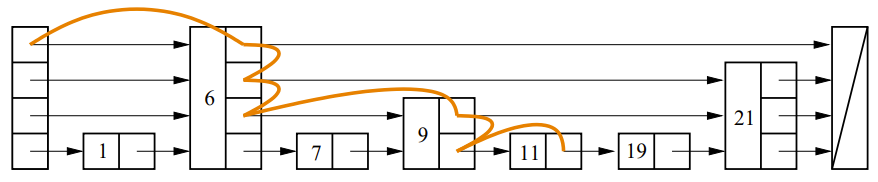
\includegraphics[width=5in]{skiplist_search.png}
\end{center}
\caption{An example traversal of a skip list (taken from Fraser (2004)'s \textit{Practical Lock Freedom})\cite{fraser2004practical}}
\end{figure}
% todo shorten to not repeat info I adapted
%During lookup, we iterate through the "upper" layers up until we see that the next element is greater than the desired key, at which point we go down to the next "lower" layer. We repeat this process until we reach the lowest layer which contains all elements, where we then find or don't find the desired item. During insertion, we follow the same lookup process (while keeping track of previous nodes in each layer). When we find the node we will be inserting after, we pick a random height (exponentially biased), and change the links in the new node and the node previous. During deletion, we similarly look up the desired node, change the pointers in each layer to skip over the deleted node, and then free the memory associated with the node.

% (Also, flexible for data distribution)
% \subsection{Skip List: An Overview}

Like its counterpart the concurrent BST, concurrent skip lists rely on randomness to achieve expected \ttt{O(log n)} operations such as search, updating, and removing. At the very worst, the skip list has \ttt{O(n)} performance for an operation, but this is extremely unlikely. This complexity is achieved through picking a random level that that node will reach to, with a bias towards lower heights. Specifically, the frequency of nodes of a particular height decreases exponentially with the height.\cite{herlihy2006provably}

% A skip list consists of a hierarchy of (logically) individual linked lists, which can be considered layers. 
\subsection{Applications}
Skip lists are often used in distributed applications as well as the underlying implementation for concurrent priority queues. Various applications can be seen from MemSQL (which uses lock-free skip lists for maintaining its indexing structure), to Redis, which uses skip lists for ordered sets.

In these applications, performance for concurrent operations is a major concern. These kinds of distributed applications often have non-independent request distributions, and might vary over time. 

We wanted to benchmark our implementations against realistic levels of contention, as further described in the Results section. After consulting with course staff we looked at implementing a pseudo-dependent workload where certain keys were chosen at random to be the most frequently called, with the PDF following Zipf's Law \cite{wikipedia_2022_Zipf}. However, without implementing a full distributed application ourselves, we would not be able to see the effects of letting specific workers have their own distributions (e.g. a producer and consumer or similar workloads) and the effect there on cache misses. When consulting the relevant literature, most papers abstracted workloads to independent identically distributed variables. We follow this standard and instead view the differences of higher or lower contention between workers by varying the distributions keys and operations are drawn from.

\subsection{Concurrent Skip Lists}
Ensuring correctness for concurrent skip lists is a significant challenge. As shown in Figure 2, it is very easy for unsynchronized insertions and deletions of nodes in a linked list to cause a "disappearing nodes" problems, where nodes inserted after a concurrently deleted node never become visible. Furthermore, unsynchronized insertions can cause a skip list to become out-of-order and thus incorrect. Throughout this project, we implement and evaluate three different implementations that resolve these correctness issues.

%\textbf{Course-grain: } Correctness of a thread-safe skip list can easily be ensured through a coarse-grained locking scheme, i.e. lock whenever an insertion, removal, or search is performed. Reader-writer locks can be used to slightly improve performance by allowing searches to occur simultaneously, but in general, this lock scheme forces insertions and removals to be done sequentially. n allow concurrent non-conflicting insertions, removals, and searches by locking only the two nodes whose pointers are updated by any given writing operation.
\begin{figure}[h!]
\begin{center}
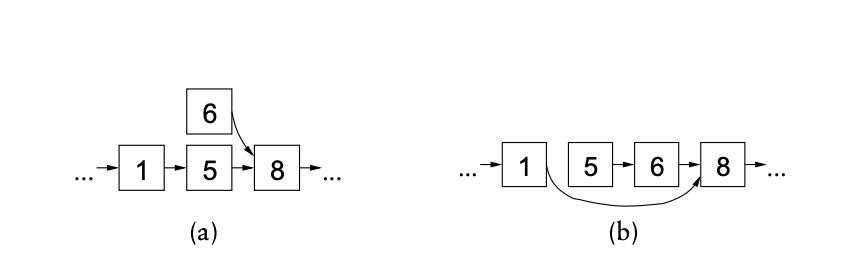
\includegraphics[width=5in]{Screen Shot 2022-05-05 at 5.58.34 PM.png}
\end{center}
\caption{Inserting key 6 while concurrently deleting key 5 results in key 6 never becoming visible, since only a deleted node points to key 6. (figure taken from \textit{Practical Lock Freedom})\cite{fraser2004practical}}
\end{figure}

After locking a given pointer, correctness is checked to ensure that the local information is the most up to date, and the pointers are unlocked after the new node has been inserted. If any other worker attempts to interact with this node, it will fail those correctness checks and retry until our current worker is done.

%\textbf{Lock-free: } Because grabbing locks itself can be expensive, particularly when this occurs repeatedly, an alternative implementation is to instead use atomic CAS operations to ensure correctness. 


\pagebreak
\section{Approach}
\subsection{Overview}
We take advantage of C++'s support for object-oriented programming, having each implementation inherit the same interface from the class \ttt{SkipList}.

 The main methods are shown below. INT\_MIN and INT\_MAX are reserved to define each end of the list, and we also require \ttt{value != nullptr} in order to use \ttt{nullptr} to indicate a key was not found.
%  Keys must be between [INT\_MIN+1, INT\_MAX-1] since INT\_MIN and INT\_MAX are reserved as the nodes at the opposite ends of the list, and the value inserted must not be nullptr, since this has a special value indicating that a key was not found.
 Our skip lists support update, removal, and lookup operations, and each skip list stores a key$\rightarrow$value mapping in each skip list node. 

\begin{listing}[!ht]
\begin{minted}{c++}
template<typename T>
class SkipList {
    public:
    /**
     * Update a mapping of key -> value, inserting the key if it is not already
     * present. The old value is returned; if the key was not present, nullptr
     * is returned. The argument "value" cannot be equal to nullptr.
     */
    virtual T *update(int key, T* value) = 0;
    
    /**
     * Remove a key from the list, return the value associated with the key.
     * If the key was not present in the list, nullptr is returned. 
     */
    virtual T *remove(int key) = 0;
    
    /**
     * Returns the value associated with a key. It returns nullptr if it is
     * not present.
     */
    virtual T *lookup(int key) = 0;
}
\end{minted}
\caption{SkipList Interface}
\label{listing:1}
\end{listing}

The main challenge of a concurrent skip list is how to ensure correctness with respect to concurrent update and removal operations. For linked list, unsynchronized insertion and deletion in a linked list can cause a new node to be inserted after a node that is simultaneously being deleted, causing the new node to never become visible because it's linked from a defunct node. Since a skip list is built upon linked lists, synchronization primitives are required to ensure that this does not occur. In general, great care is required to ensure that modifications of the skip list occur atomically and consistently. 

\subsection{Coarse-grained locking skip list}
A coarse-grained locking skip list handles correctness issues in a multi-threaded environment by ensuring that no update or removal is done concurrently and also ensures that modifications of the skip list do not occur simultaneously with reads of the skip list. We use a single mutex variable which is locked prior to an operation and then unlocked at finish. Overall, this forces all operations done to the skip list to be done sequentially and becomes a convenient baseline to compare concurrent skip list implementations.

Operations are done as they would for a skip list designed for a single-threaded environment. A lookup is done through searching through upper levels and then going down to lower levels until a key is found to be present or absent. Update and removal of nodes is done by searching at every level that pointers need to be updated. For update, the new node's pointers point to the succeeding nodes at each level, and the preceding node's pointers point to the newly inserted node. For removal, the preceding node's pointers are updated to point to deleted node's next pointers.
\subsection{Fine-grained locking skip list}
We implemented a concurrent fine-grained locking list that uses optimistic synchronization. Searches are done without acquiring locks, and short lock-based validation is used to update/insert or remove nodes atomically and consistently.\cite{herlihy2006provably} Unlike the lock-free skip list discussed in the following section, this implementation preserves skip list properties at all times and has a stronger guarantee of linearizability of operations. 
We based our implementation on Herlihy's fine-grained locking skip list pseudocode, adapting it to support values stored inside of nodes alongside the key.
% implementation?
% Note that we have slightly modified Herlihy's skip list implementation to support values stored inside of nodes alongside the key, and also that our implementation is highly based on Herlihy's pseudocode. \\
The node for our fine-grained locking skip list implementation has the following fields (methods are omitted for convenience): 
\begin{listing}[!ht]
\begin{minted}{c++}
template<typename T>
class FineNode {
    public:
    FineNode * volatile *_next; // list of corresponding next pointers
    T* volatile _value; // value associated with key
    const int _key; // integer key
    const int _top_level; // number of levels in the node (size of _next array)
    volatile bool _fully_linked; // false if an inserted node is not yet fully linked
    volatile bool _marked; // marked for deletion
    std::mutex _lock;
}
\end{minted}
\caption{Fields of the node of a fine-grained locking skip list}
\label{listing:2}
\end{listing}
Nodes are logically deleted prior to being unlinked through the "marked" variable. Regardless of linking or unlinking, an element is only considered to be in the list if the associated node is both fully-linked and not marked for deletion.

\textbf{Operations}

Lookup, update, and remove use an optimistic algorithm to search without taking locks to find the nodes that precede and succeed a given key (with \texttt{succs[0]->\_key == key} if the key exists in the skip list). This algorithm is implemented in a helper function that both returns the level at which a key is found and the predecessors and successors of the key. For lookup, we return the value stored in the node if it's not marked, fully-linked, and the level at which it was found is equal to its top\_level-1. For updates and removals, we do something else. If we update a key that is already in the list, we simply change the associated node's value and return the old value. If we remove a node that is not found in the list, we simply return nullptr (as the "previous value"). If we update a node with a key not in the list, we must insert a new node and change references. Similarly, if we remove a key found in the list, we must mark it for deletion and then unlink it.

For modification of the skip list (linking and unliking), we must perform lock-based validation. We lock predecessor nodes from the lowest level upwards, for all links that need to be modified. (This is up to the topmost level of the to-be-inserted node or the to-be-deleted node.)  We check that the predecessor nodes still point to the successor nodes and also that none of the predecessors have been marked for deletion. If it has been, we drop all locks and retry the search operation. If lock-based validation succeeds, we modify all the appropriate links (associated with nodes that we have locked). We mark a node for deletion prior to unlinking and set fully\_linked = true after successful insertion.

\begin{figure}[h!]
  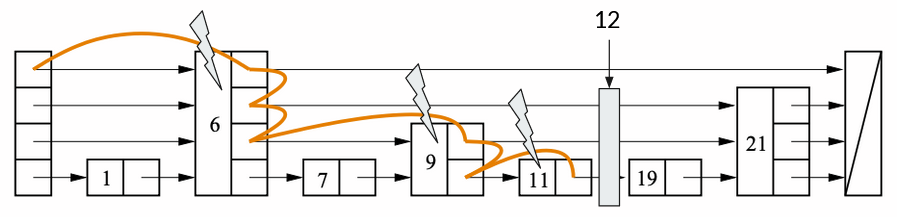
\includegraphics[width=5in]{skiplist_insertion.png}
  \caption{Insertion of a node with the key 12 and height of 3 into a fine-grained locking list. Nodes with keys 11, 9, and 6 are locked (in that order) during validation and insertion of the new node.}
\end{figure}
A key challenge of the fine-grained locking list is ensuring that deadlocks never occur. This is done through grabbing locks in a consistent order. Locks are grabbed in the order of decreasing key values, since locks are grabbed on preceding nodes from the lowest level to the topmost. Since we use lock-based validation, when we find that our values are invalid, we drop all locks and retry. Thus, we keep careful track of which locks we have grabbed and also ensure that we always drop all locks when we are retrying.

\textbf{An aside on volatile:} The volatile keyword on these shared variables is very necessary to avoid too-aggressive optimizations from a compiler that is unaware that updates to these variables can occur in another thread. Because we "retry" an operation if we find that we are attempting to modify a node marked for deletion, without the volatile keyword, the compiler interprets this as attempting to perform the same operation again without modifying any of the values that could cause us to exit the loop; thus, the compiler optimizes away the entirety of the loop entirely, into a neat one-line while true loop of an assembly instruction that jumps to itself. 
\begin{listing}[!ht]
\begin{minted}{gas}
  40368b:   eb fe   jmp 40368b <_ZN12FineLockListIiE6updateEiPi+0x10b>
\end{minted}
\caption{Incorrectly compiled assembly instruction}
\label{listing:3}
\end{listing}

Debugging this required usage of the perf monitoring tool (to determine which instruction were cycles being spent on) and then manual inspection of the assembly code. Without the volatile keyword, whenever the condition was satisfied such that this assembly instruction was run, our program would spin and no progress would be made. Initially the lack of progress seemed like it could be caused by deadlock, but was in fact a "while (true) loop" bug in the compiled code.

\subsection{Lock-free skip list}
We implemented Fraser's CAS-based design of a lock-free skip list, which uses CAS instructions to update pointers, mark nodes for deletions, and update values stored in different nodes. We implemented his pseudocode in C++ using the appropriate CAS semantics. \cite{fraser2004practical}
\begin{listing}[!ht]
\begin{minted}{c++}
template<typename T>
class LockFreeNode {
    public:
    std::atomic<LockFreeNode *>*_next;
    std::atomic<T *>_value;
    const int _key;
    const int _top_level;
}
\end{minted}
\caption{Fields of the node of a lock-free skip list}
\label{listing:4}
\end{listing}

%TODO hm not sure if i missed it, but we might want to include specific examples of what a disappearing node could look like.
\textbf{Pointer marking}: When we delete a node, we mark each next pointer, which prevents new nodes from being inserted directly after a deleted node. Since at least the lowest two bits are always zero on at least a 32-bit architecture, we use the lowest bit as a "mark" bit, where if it is 1, the pointer is associated with a logically deleted node.
%A concurrent lock-free skip list allows insertions, removals, and searches to be run simultaneously through careful usage of CAS semantics to ensure correctness. This is done through pointer marking. When a node is being deleted, the first step (after finding the node to be deleted) is to "mark" its pointers to indicate that nodes should not be inserted after the node. After this operation, preceding pointers can be changed, etc. \\

\textbf{Operations} Like Herlihy's implementation, all operations are done using a helper function \texttt{search(int key, Node **left\_list, Node ** right\_list)} which returns the predecessors and successors for a given key. \textit{Unlike} Herlihy's implementation, for the lock-free skip list, this helper function does not keep track of the level at which a key is found (unnecessary for more relaxed constraints on skip list properties) and also remove references to a nodes marked for deletion (if said node is the one being searched for). Furthermore, this helper function removes references to a deleted node if it finds a node marked for deletion while searching for a specific key.

A lookup operation just calls this helper function, checks if \texttt{succs[0]->\_key == key}, returns the associated value if so and nullptr if the key was not found. For update operations, we use said helper function to find the predecessors and successors of a given key and then use CAS operations to insert the node at appropriate levels. If the key is found, we use CAS to swap out the value for the given key. If it is not found, we insert a node by first setting the pointers of the new node to the successors and then the pointers of the predecessor to the new node. If at any point during the composite update that pointers become stale (detected through a failed CAS operation), we retry the search operation to find the new predecessors and successors of the inserted node.

For removal operations, we once again use the search helper function to find a key. If it is not found, we return nullptr. If it is found, we logically delete the key by using CAS to swap out the value for nullptr, and then we "mark" each link pointer in the node. Calling the \texttt{search()} helper function then removes all references to the deleted node. To ensure that we free this memory correctly (after no threads retain references to deleted nodes), we add this node to the \texttt{DeletionManager} class to keep track of. (This is discussed in the following subsubsection.)

\textbf{An aside on CAS:} The CAS implementation used is C++'s  \texttt{atomic\_compare\_exchange\_weak(obj, expected, desired)} function, with its default memory ordering constraint of sequential consistency. The assembly instruction it compiled into was \texttt{lock cmpxchg} on x86 architecture. Through limited testing, we found that relaxing the memory ordering constraint (e.g. to relaxed consistency) did not have an effect on performance. See our later analysis using perf to find more discussion on this matter.

\subsection{Memory Management}
Memory management is a complex issue for concurrent data structures. To have correctness, memory must not be freed while a thread retains a reference to that section of memory. If not, atomic CAS operations can get matching addresses even if the node has been deleted and recycled, and even for the fine-grained locking list, a thread might access memory that has already been recycled. To conserve time and quickly move onto performance measurements, we chose a very simple, memory-inefficient (but correct) method of manual memory management: We do not free memory of deleted nodes at the time of deletion. Instead, we rely on the user to call \texttt{cleanup()} (or delete the overall skip list) at some point that threads do not retain any memory accesses to delete nodes (e.g. all insert and deletion operations have finished).

Manual memory management is implemented through the class \texttt{DeletionManager} which maintains an array of pointers to deleted nodes. Every time a node is removed from the skip list, instead of the memory being freed, a pointer to said memory is put in the array; the index into the array is determined through an atomic "counter" variable. Thus, we need to know the maximum number of deleted nodes at a given time at the time of instantiating the skip list.

We use this \texttt{DeletionManager} for both the lock-free skip list as well as the fine-grained locking list, and we ran a number of test cases using valgrind to ensure that memory is accessed and freed correctly, and no memory leakage occurs. The coarse-grained locking list does not require this kind of memory management because other threads cannot retain references to a node in the skip list after it has been removed, since only one thread can perform an operation (lookup, update, removal) on such a skip list at a time.
\pagebreak
\section{Results}
\subsection{Input Distributions}
In considering our input distributions we wanted to model how our skip list implementations would act across various workloads. It's very likely that certain regions of the list are more heavily "desired" by different threads, and thus have higher contention.

While course-grained locking will have contention no matter where the concurrently requested keys are in the list, we were interested in seeing how our lock free and fine lock implementations handled situations where nodes with the same or adjacent keys were concurrently inserted or deleted.
% Because skip lists are linked lists relying on the validity of their parents, 
%TODO add more here

We benchmarked our performance across implementations for a few different simulated workloads. We define a workload based on these parameters: what the ratio of update/remove/lookup operations was, what key distribution was used, and how populated the list was before we benchmarked our code.

The following benchmark visualizations were taken on the GHC machines. We created the key and operation inputs before timing our implementation. Each were initialized in vectors where each element was selected independently according to their distribution. E.g. as seen below, when using a normal distribution with a mean of 0 and a variance of 1000 for the keys, and \ttt{update\_prob=.1,remove\_prob=.1}, as the operation parameters, every time-step had probability $.8$ of being a lookup, $.1$ of being an update, and $.1$ of being a remove, as well as being called with a key drawn independently from \ttt{Normal(0,1000)}. 

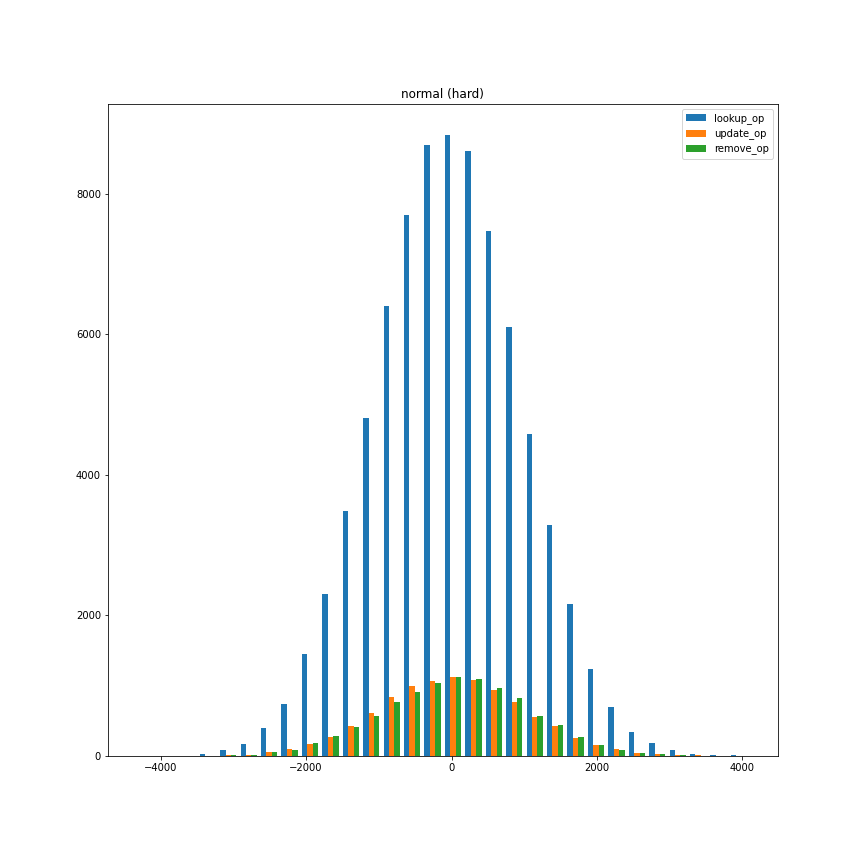
\includegraphics[width=5in]{normal_hard_byop.png}
% While we considered varying distributions based on what operation was happening, 

All benchmarking statistics in this section were taken with 1 million operations, except for the key histograms which use 100,000 for simplicity.

When experimenting with workloads we realized that high-lookup workloads were running quite quickly because we were benchmarking starting at empty skip lists. If we had $10\%$ updates/inserts and $90\%$ lookups, by the 1000th operation we would only have 100 items in our list, and a lot of trivial lookup operations.
Similar to how we need to warm up the cache to get a better approximation of performance in the long run, when benchmarking data structures we also need to warm up that structure to make tests adequately difficult.

\textbf{Key Distribution} \\
We looked at Normal, Uniform, and Bimodal (Mixed Normal Distributions) distributions, and wanted to look at two "difficulties" associated with each. For easy, the warm up inserts were run with half the array length (500k) and keys drawn from the same distribution as the timed run. 

% TODO(grace): check
% Because levels for nodes in the skip list are chosen randomly, the data structure can approximate \ttt{log(n)} search with any d
Because the nodes in the list are distributed according to the key distribution, having the same workload/distribution throughout data structure lifetime ensures the expected O($\log n$) time complexity. However, we wanted to see what happens with contention when that higher level of key frequency is not accounted for in the structure. Our hard versions have 2 million keys randomly inserted uniformly (within roughly 2 * the standard deviation on either side) during warm up. If the "highway" nodes \ttt{A} and \ttt{B} are far apart due to the even PDF of the warm up round, but have a number of concurrent operations to the same or neighboring keys, that would cause contention.
For readability the remaining key distribution graphs will combine all operation types. 
[500,000 $\leftarrow$ \ttt{Normal(0,1000)}] would mean that 500,000 keys are generated independently from the normal distribution with mean of 0 and variance of 1000. 

Let \ttt{U = Uniform}, \ttt{N = Normal}, \ttt{B(m1,m2,v) = .6 * N(m1,v) + .4 * N(m2,v)}, or an averaging of the two distributions. Let \ttt{S = } $2 * \sqrt{1000}$. We note that with the decreased distance between means, the bimodal chart approximates a normal distribution.

\begin{table}[ht]
\begin{center}
\begin{tabular}{|c | c | c|}
 \hline
 Graph & warmup & timed \\ 
 \hline \hline
 \hline
 Normal (easy) & \ttt{[}$500,000 \leftarrow$ \ttt{N(0,1000)]} & \ttt{[}$1,000,000  \leftarrow$ \ttt{N(0,1000)]} \\
 \hline
 Bimodal (easy) & \ttt{[}$500,000 \leftarrow$ \ttt{B(-1000,1000,250)]} & \ttt{[}$1,000,000  \leftarrow$ \ttt{B(-1000,1000,250)]} \\
 Uniform (easy) & \ttt{[}$500,000 \leftarrow$ \ttt{U(-1000,1000]} & \ttt{[}$1,000,000  \leftarrow$ \ttt{U(-1000,1000)]} \\
 \hline
 Normal (hard) & \ttt{[}$2,000,000 \leftarrow$ \ttt{U(-S,S)]} & \ttt{[}$1,000,000  \leftarrow$ \ttt{N(0,1000)]} \\
 \hline
 Bimodal (easy) & \ttt{[}$2,000,000 \leftarrow$ \ttt{U(-S,S)]} & \ttt{[}$1,000,000  \leftarrow$ \ttt{B(-S,1000,250)]} \\
 Uniform (easy) & \ttt{[}$2,000,000 \leftarrow$ \ttt{U(-1000,1000]} & \ttt{[}$1,000,000  \leftarrow$ \ttt{U(-1000,1000)]} \\
 \hline
\end{tabular}
\label{table:2}
\caption{Table of perf stats inputs on randomized keys from range 200,000}
\end{center}
\end{table}


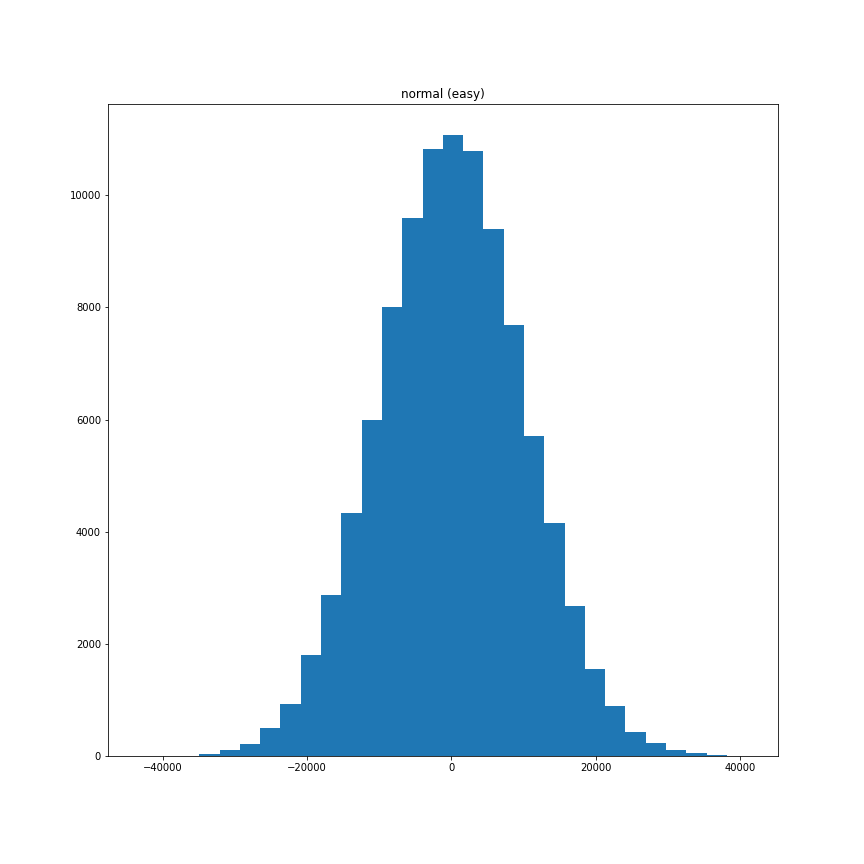
\includegraphics[width=3.4in]{normal (easy).png}
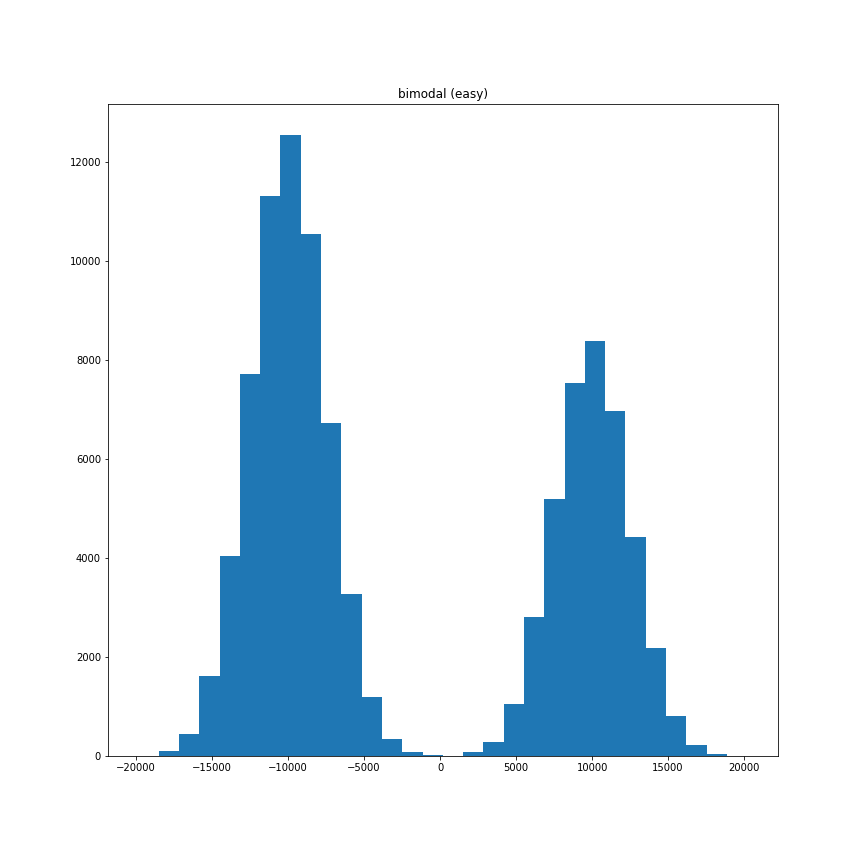
\includegraphics[width=3.4in]{bimodal (easy).png}
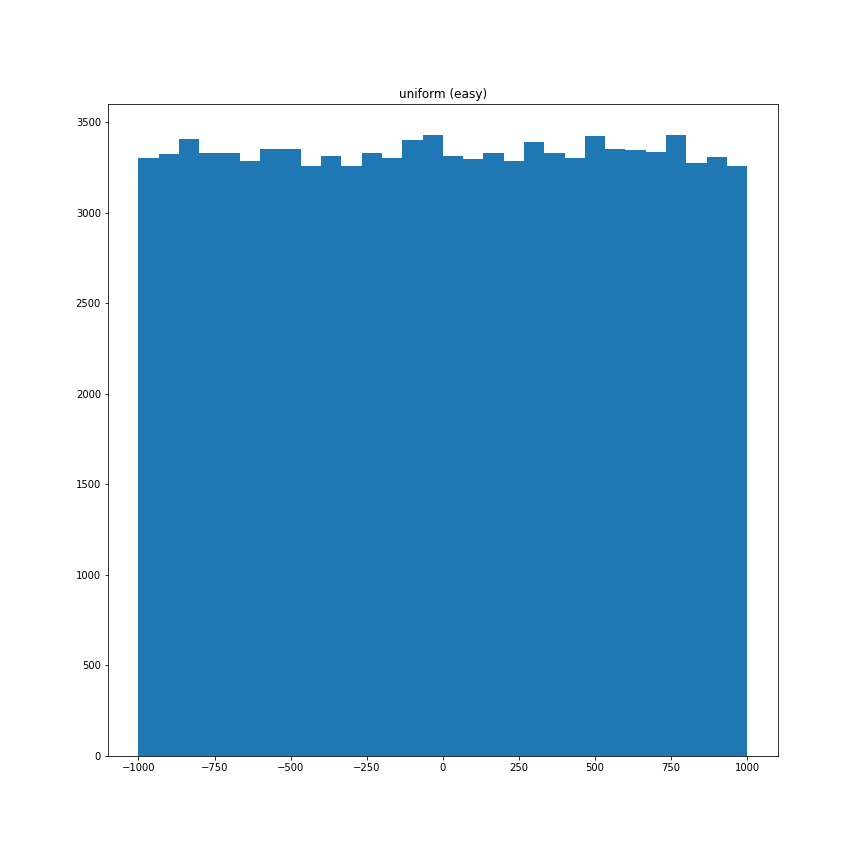
\includegraphics[width=3.4in]{uniform (easy).png} \\
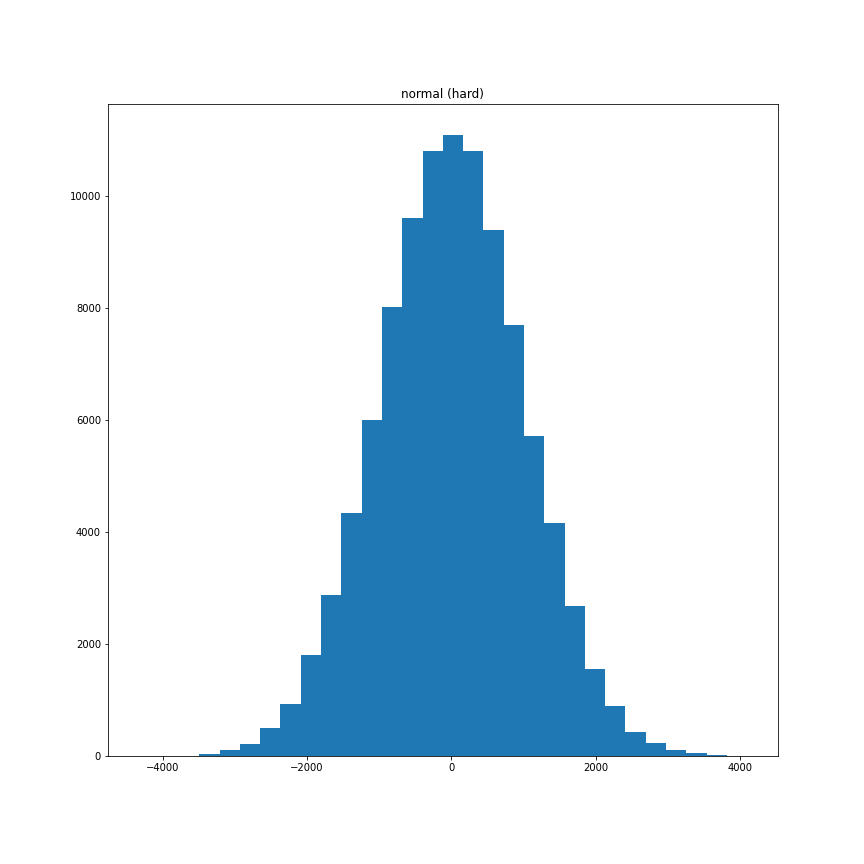
\includegraphics[width=3.4in]{normal (hard).png}
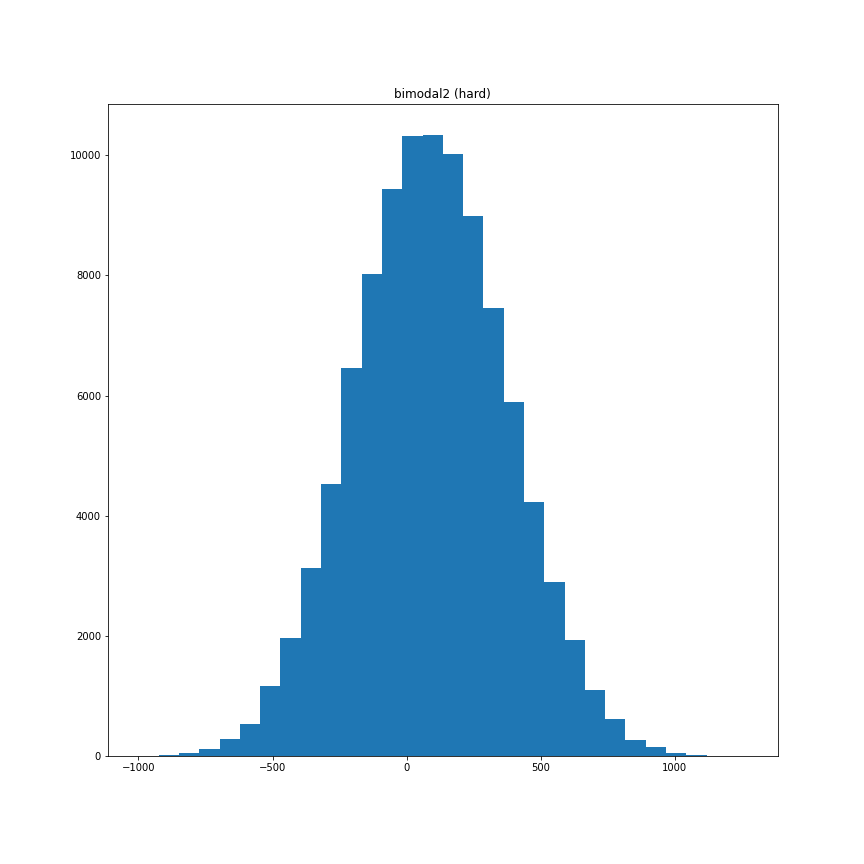
\includegraphics[width=3.4in]{bimodal2 (hard).png} \\
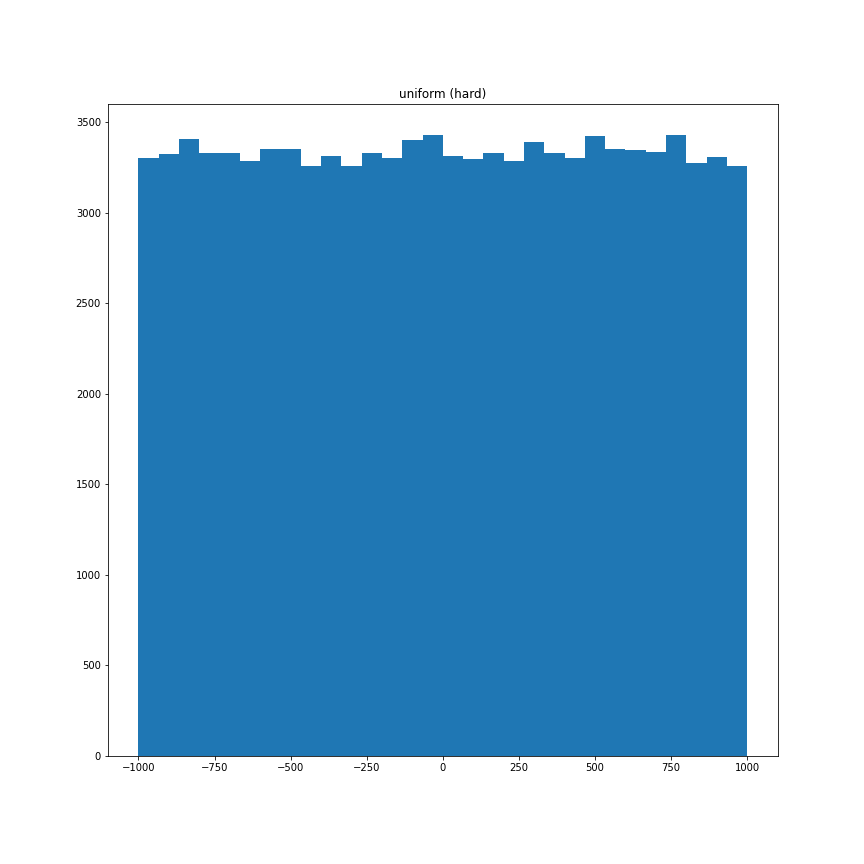
\includegraphics[width=3.4in]{uniform (hard).png}
% \begin{figure}[h!]
%   \caption{A picture of the universe!}
%   \includegraphics[width=0.5\textwidth]{universe}
% \end{figure}

% \begin{figure}	
% 	\centering
% 	\begin{subfigure}[t]{3in}
% 		\centering
% 		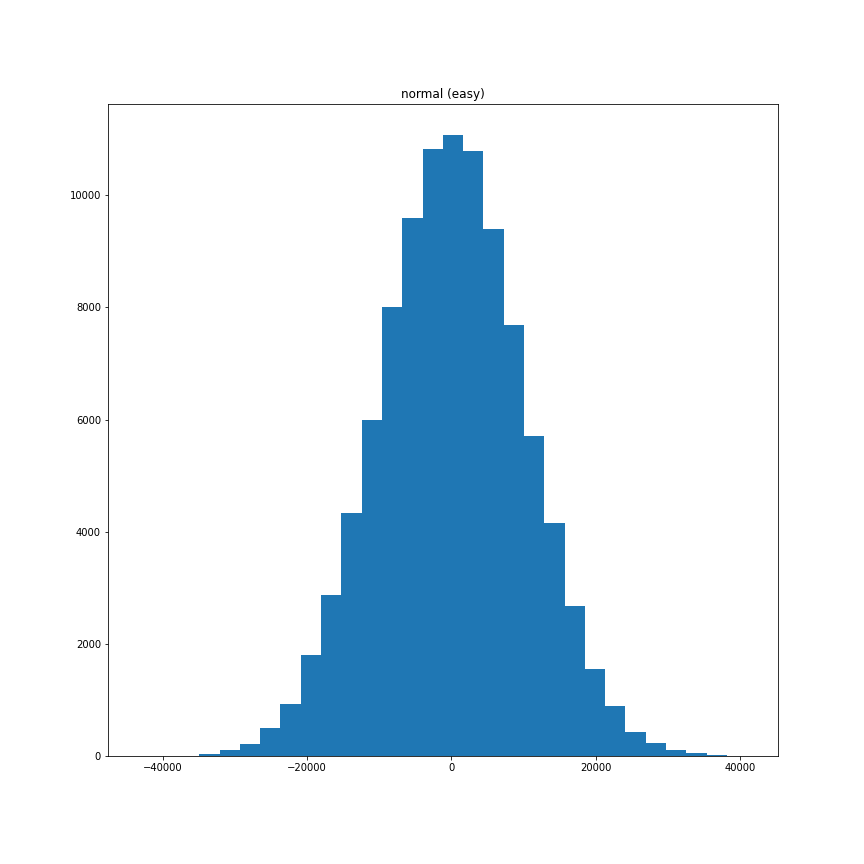
\includegraphics[width=3in]{normal (easy).png}
% 		\caption{W = [500,000 \leftarrow Normal(0,1000)], T = [500,000 \leftarrow Normal(0,1000)]}\label{fig:1a}		
% 	\end{subfigure}
% 	\quad
% 	\begin{subfigure}[t]{1in}
% 		\centering
% 		\includegraphics[width=1in]{placeholder}
% 		\caption{Caption 2}\label{fig:1b}
% 	\end{subfigure}
% 	\caption{Main figure caption}\label{fig:1}
% \end{figure}

% % \textbf{All graphs}

\textbf{Other input notes}
We looked at how throughput varied across workload for our different implementations. 

The results are in accordance with our expectations. Here is a sample of two: \\
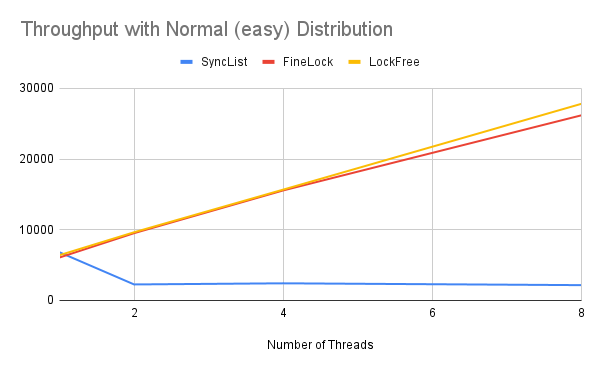
\includegraphics[width=3.2in]{Throughput with Normal (easy) Distribution.png}
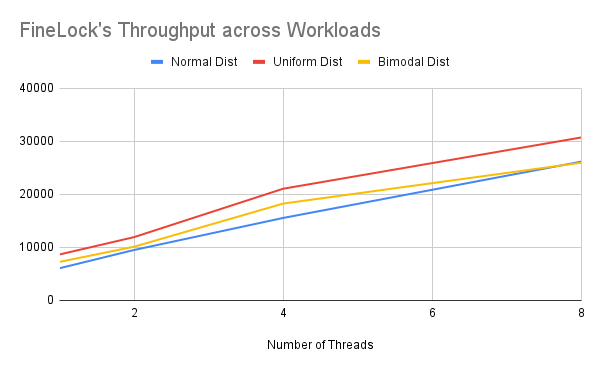
\includegraphics[width=3.2in]{FineLock's Throughput across Workloads.png}

Because we care more about the difference between data structures than overall speedup (as skip lists tackle a difficult concurrency problem), the majority of our performance evaluation will be comparing LockFree and FineLock to SyncList. SyncList completely fails to achieve any speedup across multiple threads, since the coarse-grained locking scheme forces all operations to happen sequentially. However, the other two implementations allow a high number of concurrent operations. As expected, workloads that involve less contention (lesser likelihood that the same or neighboring nodes are concurrently modified) have better throughput. \\
\textbf{Distribution Effect} \\
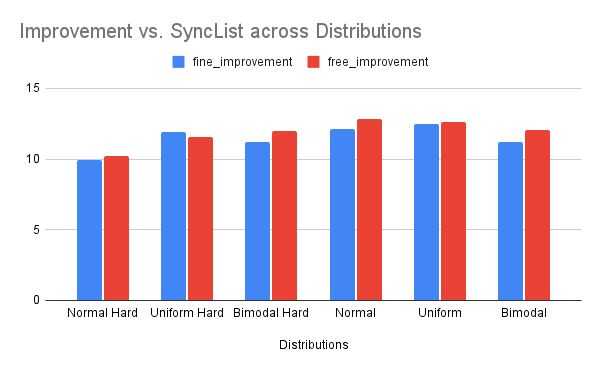
\includegraphics[width=5in]{Improvement vs. SyncList across Distributions.png} \\
You can see this overall from the above figure, where we plot the "speedup" when moving from a SyncList Implementation on 8 threads to a FineLock/LockFree Implementation on 8 threads. This was calculated on the GHC machines by dividing the average time the SyncList took on the given workload by the average time for each respective improved implementation.
We get up to 10x relative improvements, and the benefit is pretty similar across the two better implementations. 

Because the harder distributions will give the different workers more nodes to traverse and potentially get delayed on, we expected to see more results of contention dividing our different implementations. However as discussed earlier, sync list is pretty uniformly bad as it always locks regardless of key proximity. Both our improved implementations do have less of a speedup compared to the SyncLock in these harder distributions, which makes sense given that these will have more dependencies and more necessary latency to ensure correctness.

Between the two implementations the speedup is pretty similar, although LockFree tends to slightly edge out SyncList. Additionally, the overall robustness across implementations for these workloads suggest that both of these are pretty similar for independent identically distributed workloads similar to the ones we tested. As mentioned in Herlihy (2006), this supports the idea of FineLock having comparable performance as the LockFree list with a simpler implementation and stronger skip list property guarantees.\cite{herlihy2006provably}
% TODO include or not?
%We also considered giving different operations different distributions, but our skiplists were mostly resistant to system wide distribution changes, decided it would be better to spend time on more analysis of other workload variations.
\subsection{Performance Measurements}
We also performed performance measurements on the PSC machines. On a skip list (initially inserted with 500,000 keys selected from the respective key distribution), we performed 1,000,000 operations: lookups, updates, and removals with different probability. The keys associated with said operations were selected from a uniform distribution of size 2,000,000 or 200,000. We used OpenMP to parallelize a for loop on the appropriate number of threads, and we compared performance across different numbers of threads (1, 4, 16, 64, or 128). Throughput was measured as taking the number of operations (1,000,000) and dividing by the total runtime of said operations. We tested on different update, removal, and lookup distributions, mimicking Herlihy's performance measurements of their fine-grained locking skip list.\cite{herlihy2006provably} 

\begin{figure}[h!]
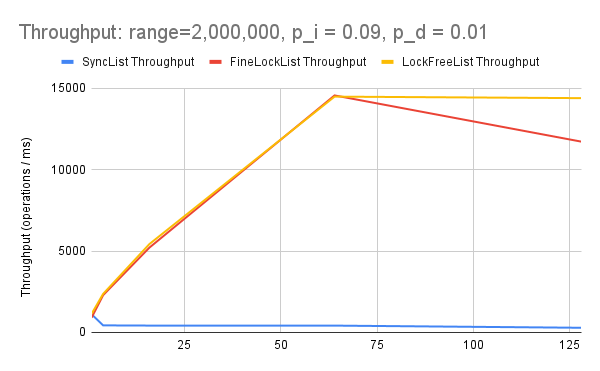
\includegraphics[width=3.4in]{Throughput range=2,000,000, p_i = 0.09, p_d = 0.01.png}
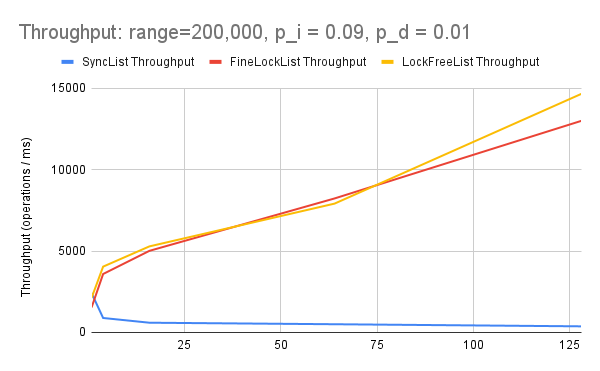
\includegraphics[width=3.4in]{Throughput range=200,000, p_i = 0.09, p_d = 0.01.png}

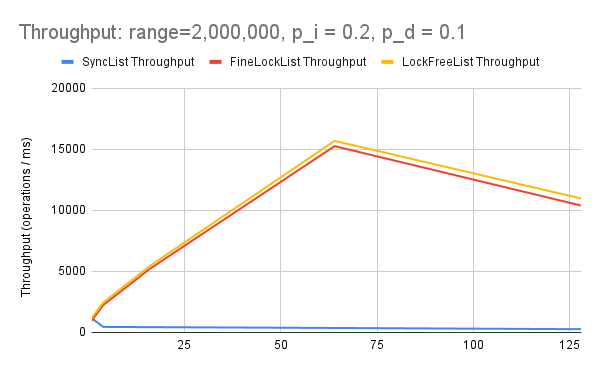
\includegraphics[width=3.4in]{Throughput range=2,000,000, p_i = 0.2, p_d = 0.1.png}
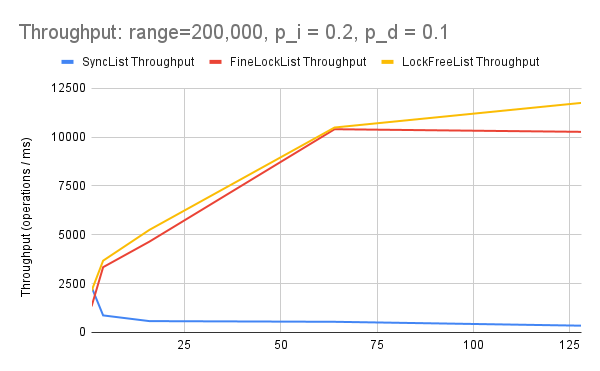
\includegraphics[width=3.4in]{Throughput range=200,000, p_i = 0.2, p_d = 0.1.png}

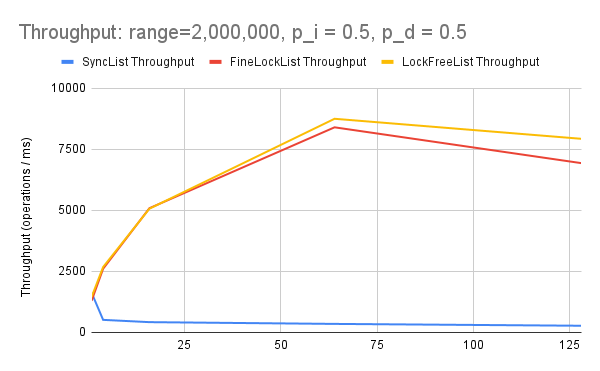
\includegraphics[width=3.4in]{Throughput range=2,000,000, p_i = 0.5, p_d = 0.5.png}
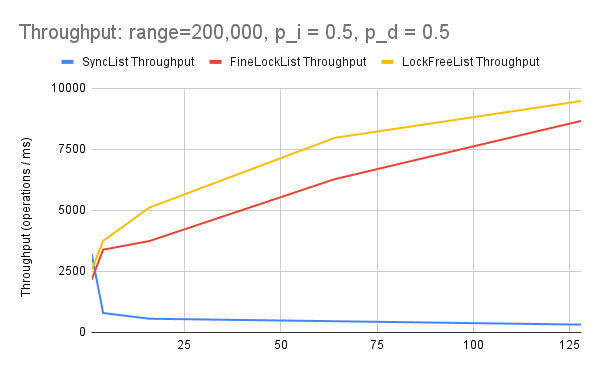
\includegraphics[width=3.4in]{Throughput range=200,000, p_i = 0.5, p_d = 0.5.png}
\caption{Performance benchmarking on the PSC machine on uniform key distributions with different probabilities of update/insertion ($p_i$) and removal/deletion ($p_d$). The reset of the operations are lookups. }
\end{figure}
\textbf{Evaluation of concurrent skip list:} As shown in the graphs and in accordance with our expectations, we find that both the fine-grained locking skip lists and lock-free skip lists offer substantial performance improvement as compared to the coarse-grained locking implementation. Very few skip list operations can be done per second on a coarse-grained skip list, since all operations must be done sequentially; however, depending on the workload (proportion of insertions, deletions, etc.), we can achieve close to 7,500 to close to 15,000 operations per millisecond at maximum, since these operations can be done concurrently.

\textbf{Effect of contention:} As we expected, the throughput varies depending on the contention caused by the distribution. With keys selected from a uniform distribution of 2,000,000, it is more unlikely for concurrently running threads to be updating, looking up, and/or removing keys that are adjacent and/or the same. However, with a smaller key distribution of range 200,000, we have contention, which means that operations need to be retried if lock-based validation fails (for the fine-grained locking implementation) or if pointers become stale (for the lock-free implementation). When we perform operations with a smaller range of keys, even though the skip list operated on is smaller (with keys selected from 200,000 integer values instead of 2,000,000), we have a lower throughput of operations in a concurrent environment.

\textbf{Comparing fine-grained and lock-free:} We also find that the fine-grained locking list has a very similar performance to the lock-free skip list. This is in accordance with Herlihy's performance measurements for their implementation. Herlihy found that their skip-list algorithm (implemented in Java) had similar performance but a slight advantage over Doug Lea's nonblocking skip-list implementation in almost all scenarios.\cite{herlihy2006provably} In contrast, our measured numbers indicate that our implementation (in C++) of Herlihy's fine-grained locking skip list has similar performance but a slight \textit{disadvantage} over the lock-free skip list in almost all scenarios. This is expected because we implemented Herlihy's implementation almost directly from their pseudocode, which was optimized for simplicity, not efficiency. We did not implement Herlihy's optimizations, such as not looking further if a node with an appropriate key is found, or having search start from the highest \textit{non-empty} layer. We could have also stored the bool variables fully-linked and marked in other fields (such as the lowest bits of the pointers), to minimize the memory usage and the required number of memory accesses. This was one advantage our lock-free skip list had over our fine-grained locking skip list.

Performance of the fine-grained locking skip list only degrades and is significantly less that of the lock-free skip list under very high contention, e.g. the case with update and deletion probability both equal to 0.5, and the range of values is only 200,000. We expect that this fine-grained locking list implementation would be worse than the lock-free list under contention. Both skip lists have very similar retry mechanisms. Validation only succeeds whenever the predecessors seen during the search phase are unchanged before they are locked or attempted to be modified by CAS operations, for the fine-grained locking skip list and lock-free skip list respectively. They both retry, so they have nearly identical overall trends. However, the fine-grained locking skip list has the additional overhead of acquiring and releasing multiple locks on every retry, which explains its lower performance under identical levels of contention.

\textbf{An aside on performance degradation at high thread count}: One might notice that throughput levels out or decreases going from 64 to 128 threads for operations on keys selected from a uniform distribution of range 2,000,000. This is in fact indicative of where our throughput abstraction falls apart. At high thread counts, the overhead of OpenMP and our benchmarking code itself becomes significant, obscuring the benefits of performing concurrent operations. This is supported by running perf on the PSC machines on these inputs. As shown in the following figure, a shocking $\geq$30\% of overall cycles are spent on the OpenMP code; furthermore, a surprising 18\% of cycles are spent loading memory from the keys and ops vectors we used to store our randomized keys and operations (as is done in \ttt{perform\_test}).
\begin{figure}[h!]
  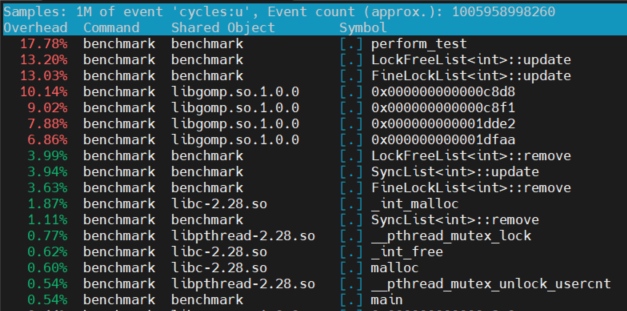
\includegraphics[width=5in]{psc_benchmark_cycles.png}
  \caption{distributions of cycles measured using perf record on benchmark on 128 threads, 2,000,000 range, $p_i$ = 0.5, $p_d$ = 0.5}
\end{figure}

\textbf{Speedup (fine-grained locking and lock-free list over coarse-grained locking}: Performance of the fine-grained locking and lock-free skip list can also be determined relative to the coarse-grained locking skip list by dividing the runtime of operations executed on the coarse-grained locking skip list by the runtime on the other two skip lists. Through the implementation and usage of more concurrent data structures, we can perform up to 40x more operations on concurrent skip lists through multi-threading. We also find that we have better speedup / more capability for concurrent operations when we have less contention, e.g. the range of keys is larger and the probability of updates and removals is smaller, so it is less likely for threads to be attempting to modify the same or neighboring nodes. 
\begin{figure}[ht]
  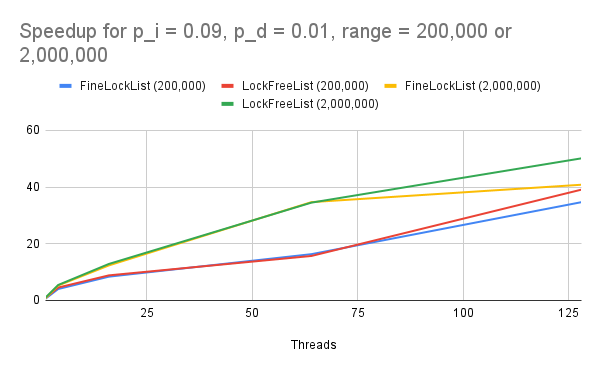
\includegraphics[width=3.4in]{Speedup for p_i = 0.09, p_d = 0.01, range = 200,000 or 2,000,000.png}
  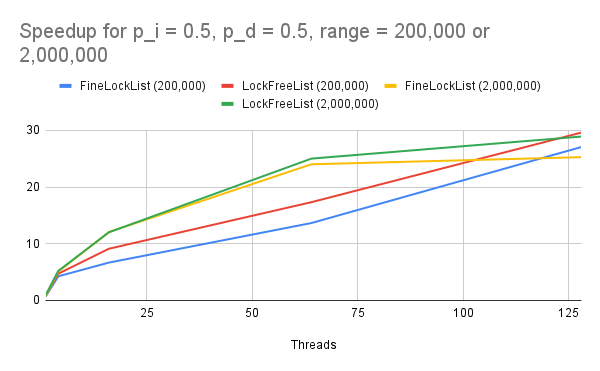
\includegraphics[width=3.4in]{Speedup for p_i = 0.5, p_d = 0.5, range = 200,000 or 2,000,000.png}
  \caption{Speedup of fine-grained locking and lock-free skip lists over the coarse-grained skip list on PSC benchmarks}
\end{figure}

\pagebreak
\subsection{Performance Analysis under contention}
We used a contrived example to test the performance of our skip lists under extremely high contention. On the GHC machines, we inserted and removed a node with the same key and a height of 20 (ensured by setting the probability of increasing the level of the skip list as 1 and setting the maximum height of the skip list as 20). We performed 1,000,000 operations, 50\% update and 50\% remove operations, parallelized through OpenMP across eight threads. We ran the same test inputs on all three skip lists, using perf stat and perf record, recording the inputs cycles, instructions, cache-misses, and cache-references. For perf stat, we ran the same workload 5 times to collect combined statistics, but we did not do so for perf record since it does not has similar functionality. \\

\textbf{Collected statistics:}
\begin{table}[h!]
\begin{center}
\begin{tabular}{|c c c c|}
 \hline
 Statistic & Coarse-grained locking & Fine-grained locking & Lock-free \\ 
 \hline \hline
 \hline
 Cache misses & 560,688 & 2,265,229 & 1,616,294 \\
 \hline
 Cache references & 35,048,524 & 14,774,453 & 546,798,257 \\
 \hline
 Miss rate & 0.383\% & 15.332 \% & 0.296\%\\
 \hline
 Cycles & 1,815,444,699 & 5,260,737,615 & 10,053,581,967 \\
 \hline
 Instructions & 1,318,406,323 & 9,182,573,505 & 2,203,105,075 \\
 \hline
 IPC & 0.73 & 1.75 & 0.22 \\
 \hline
 Elapsed time & 0.5338 & 0.7158 & 1.0010 \\
 \hline
\end{tabular}
\label{table:4}
\caption{Table of perf stats inputs on a single key inserted and removed 1,000,000 times}
\end{center}
\end{table}

As shown in this table, the behavior of all three skip lists differs highly when under contention. As expected, the coarse-grained locking list has the best behavior under contention. Because each time we are inserting and removing the same node, we cannot do any better than sequentializing the program, since this unlinking and relinking of the node must be done atomically. Thus, coarse-grained locking has better performance than either fine-grained locking or lock-free lists. 

\textbf{Coarse-grained locking versus other skip lists:} Furthermore, during update or removal, if the nodes are modified during the optimistic search process of finding the predecessors and successors to a node, both the lock-free and fine-grained locking lists "retry" the operation, starting over and performing another optimistic search. From the perf stats, we can see that this happens from the much higher instruction counts for both the fine-grained locking and lock-free lists; the operations are retried a number of times.

This higher number of "retries" can be shown by using perf record to check the instruction percentages. In the coarse-grained locking skip list, we only have about 30\% of total instructions in update and remove operations. In the fine-grained locking skip list, we have about 60\% of total instructions in update and remove operations, and in the lock-free skip list, we find that we have about 50\% (removal) of total instructions in update and removal operations. From a closer analysis of the code, we find that most of these instructions in said update and removal functions are in the instructions involving searching the list. This confirms our expectation that repeated "retries" cause both the fine-grained locking and lock-free skip lists to perform worse than the coarse-grained locking list. 

\begin{figure}[h!]
  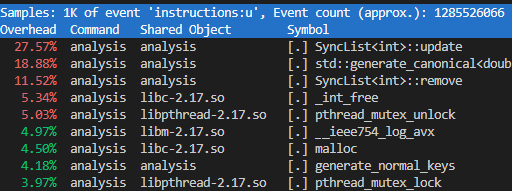
\includegraphics[width=5in]{ex2_s0_instructions.png} \\
  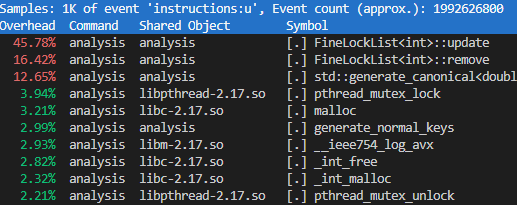
\includegraphics[width=5in]{ex2_s1_instructions.png} \\
  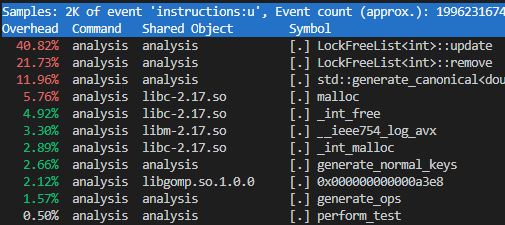
\includegraphics[width=5in]{ex2_s2_instructions.png}
  \caption{Perf record results of instruction percentage for three skip lists on a contrived high-contention use case. From top to down is coarse-grained locking, fine-grained locking, and lock-free skip lists. }
\end{figure}

\textbf{Lock-free versus Fine-grained locking:}
Unexpectedly, we find that under this contrived use case, the lock-free skip list has worse performance than the fine-grained locking skip list, with the same number of skip list operations taking more time than that of the fine-grained locking skip list. This is especially unexpected because we know that the fine-grained locking skip list retries operations much more times than the lock-free skip list (as shown by the associated much higher instruction count) and yet the lock-free skip list takes many more cycles due to its much, much lower IPC. 

The performance of the lock-free skip list is very difficult to understand, especially because the cache \textit{miss} rate associated with the lock-free skip list is also lower than that of the fine-grained locking list, so the miss rate does not explain the degradation in performance. When using perf record to find the cycle-heavy instructions, the issue becomes apparent: the \texttt{lock cmpxchg} instruction, which involves a disproportionate number of both the total cycles and cache references (which the lock-free skip list also has an unusually high number of). In the lock-free skip list, \texttt{lock cmpxchg} instructions appear multiple times (marking pointers for deletion, removing references to a deleted node, and also adding references to an inserted node), and each has a disproportionately high rate of cycles and cache references. These \texttt{lock cmpxchg} instructions compile from the compare-and-swap instructions. To perform the required atomic write involved in a compare-and-swap, \ttt{lock cmpxchg} locks the cache line for modification, which means that other processors must stall until the other processors are done modifying the data in order to likewise access the data for modification. This cache coherence traffic and number of stalls from the overhead of atomic instructions are the reason why in this excessively high contention use case, the lock-free skip list performs the worst of all three skip lists. 

\begin{figure}[h!]
  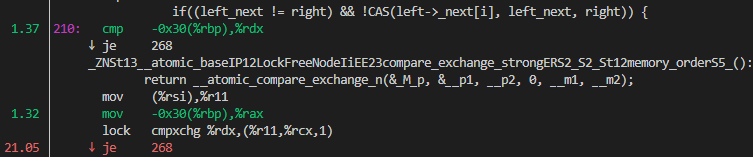
\includegraphics[width=5in]{ex2_s2_cache_references.png} \\
  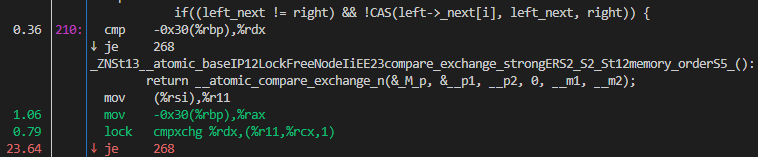
\includegraphics[width=5in]{ex2_s2_cycles.png}
  \caption{perf record results for lock-free skip list on a contrived high-contention use case. Both images show the same instructions which are involved in removing references to a deleted node. Above shows the high rate of cache references involved in the lock cmpxchg instruction, and below shows the high rate of cycles associated with the lock cmpxchg instruction.}
\end{figure}

The fine-grained locking list does not run into this problem because instead of atomic instructions, it uses locks to guard data and prevent concurrent modification of shared variables. In this case, the locks prevent the high amount of cache coherence traffic and stalling for cache lines modified by other processors that is caused by the alternative use of atomic variables.

However, this performance difference does not show up in any of the use cases discussed in the previous section. So why does the lock-free skip list perform better than the fine-grained locking list in almost all cases in our previous performance measurements on the PSC? This is because this scenario is especially contrived since it results in multiple processors competing for the exact same cache line, which is very rare in non-contrived use cases for concurrent skip lists. In general, users of a skip list will insert and remove more than one node and usually not the same node, so contention is generally much rarer than this contrived use case. When contention occurs, processors will spend more time searching than directly operating on the same pointers that are modified across different processors. Furthermore, when a node of the skip list has a smaller height (which is exponentially biased by a skip list), fewer variables are atomically modified (to add or remove references to the node), further decreasing the likelihood of reading a variable being atomically written to by another processor.

Instead, it is more likely for pointers to be changed between the time of searching the list to find predecessors and successors to the node and the time of modification of said pointers. This results in retries of the search for both fine-grained locking and lock-free skip lists, which is similarly expensive for both. However, this failure of validation is more expensive when using the locks taken by the fine-grained locking list. This is in contrast to the overhead of atomic variables in the much, much unlikelier scenario of multiple processors trying to atomically write to the exact same pointers. 

Additionally, this test was performed on the GHC instead of the PSC machines. We expect that the cost of atomic operations is highly architecture-specific (due to the cost being dependent on the implementation of cache coherence) which makes it difficult to compare different test cases across different machines. 
\pagebreak
\subsection{Execution time breakdown with perf: Lower contention and more general use cases}
% Show measurements and analysis from perf report
We also performed a test case on perf that was more similar to a usual workload to analyze a different scenario. Our test inputs were 10,000,0000 operations (40\% update, 40\% remove, 20\% lookup) with randomized keys from a uniform distribution of range 200,000. As before, these operations were done in parallel on eight threads, with thread scheduling by OpenMP using "dynamic" scheduling on the GHC machines. We ran the same test inputs on all three skip lists, using perf stat and perf record in the same way. \\
%From a high-level perspective, we expect that operations on our skip list are  memory-bound. Lookups, insertions, and removals have very few arithmetic operations (only comparing integer keys for each node) and very frequent memory accesses (to traverse the list through pointers). Furthermore, we expect that memory accesses are especially expensive due to poor locality in memory accesses, since a concurrent skip list does not occupy contiguous locations in memory, but rather accesses occur in different sections of memory provided by the memory allocator. %We also expect that under high contention, the effect of locks for the fine-grained locking implementation is more significant than that of memory accesses, and also that the number of retries for both implementations will dominate. \\
%Using the performance monitoring tool perf, we found that instructions that took most of the total cycles were also the instructions that caused most of the cache misses, i.e. the instructions used to traverse the skip list. However, the cache miss rate was especially low for all three implementations, which indicates that our performance bottleneck may be something else. In particular, our performance bottleneck may be the low instruction-level parallelism in key parts of our code. 
\textbf{Collected statistics:}
\begin{table}[ht]
\begin{center}
\begin{tabular}{|c c c c|}
 \hline
 Statistic & Coarse-grained locking & Fine-grained locking & Lock-free \\ 
 \hline \hline
 \hline
 Cache misses & 446,485 & 1,140,939 & 380,681 \\
 \hline
 Cache references & 116,510,375 & 128,055,770 & 156,286,513 \\
 \hline
 Miss rate & 0.383\% & 0.891\% & 0.244\% \\
 \hline
 Cycles & 1,820,390,492 & 1,910,183,275 & 2,093,867,708 \\
 \hline
 Instructions & 822,925,365 & 962,799,069 & 1,129,300,603 \\
 \hline
 IPC & 0.45 & 0.5 & 0.54 \\
 \hline
 Elapsed time & 0.45774 & 0.083778 & 0.08771 \\
 \hline
\end{tabular}
\label{table:1}
\caption{Table of perf stats inputs on randomized keys from range 200,000}
\end{center}
\end{table}

From these statistics collected using perf stat, we find that the coarse-grained locking list took the least number of cycles and instructions but had the highest elapsed time. This is expected for a multi-threaded use case, since this entire instruction stream was forced to be sequential, unlike for the fine-grained and lock-free skip lists. We find that our cache miss rate remains quite low at less than 1\% for all skip lists. The lock-free skip list had the lowest number of cache misses (possibly due its lack of mutex locks), while the coarse-grained locking list had fewer cache misses than the fine-grained locking list. The fine-grained and lock-free skip lists have highly similar execution time, which is expected on this use case with relatively low contention. 

On all three lists, we found that list traversal took most of the cycles (i.e. searching for a requested key, either for lookup, update, or deletion). This is expected because it is the primary component of the algorithm, and it has both a memory cost and very low instruction-level parallelism. We require several memory accesses to non-contiguous locations in order to traverse a skip list. Furthermore, this process has a high level of dependency between instructions. When traversing a list, we need to have loaded the current node's \ttt{\_next} pointers into a register to load the next node's \ttt{\_next} pointers into a register, and so on. This confirms the design direction of the both fine-grained locking and lock-free skip lists. We find that it is optimal for both those data structures to make it possible to run as concurrently as possible, with list searching done in parallel without locks (for the fine-grained locking list) and usually without compare-and-swaps (for the lock-free skip list). \\
\textbf{Coarse-grained locking skip list:} \\
\begin{figure}[h!]
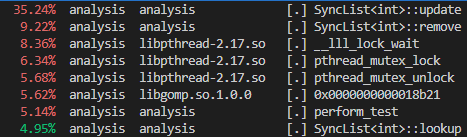
\includegraphics[width=3.4in]{ex1_s0_overall_cycles.png}
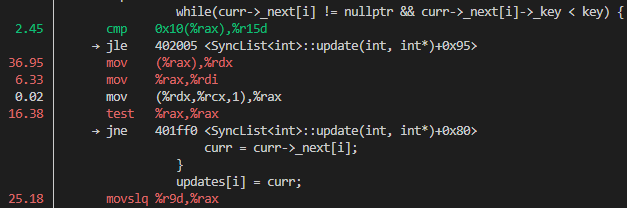
\includegraphics[width=3.4in]{ex1_s0_cycles.png} \\
\caption{perf record results for the coarse-grained locking skip list on a 10,000,000 operations done on keys in a 200,000 range. From top to bottom is the cycle percentage between different functions, and then a "zoomed in" screenshot of instructions with more cycles}
\end{figure}
%From analysis using perf, we find that the instructions that used the most cycles were also the instructions that had the most cache misses, which could be because proportionately these instructions were executed more often.
From analysis using perf, we see that the skip list traversal instructions have proportionately the most cycles. For both functions with the highest numbers of cycles (update() and remove()), we find in both cases that the greatest percentage of cycles is spent on skip list traversal--comparing keys, loading the next pointer into a register, etc. We also notice that mutex locking and unlocking is an expensive operation; around 14\% of cycles in spent on such operations, when about 50\% of total cycles are spent on update, removal, and lookup. 

\textbf{Fine-grained locking skip list:}
\begin{figure}[h!]
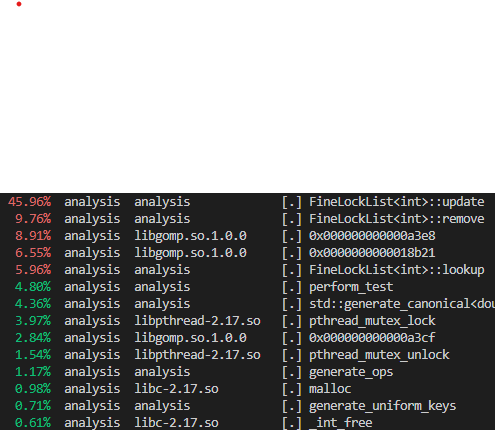
\includegraphics[width=3.4in]{ex1_s1_overall_cycles.png}
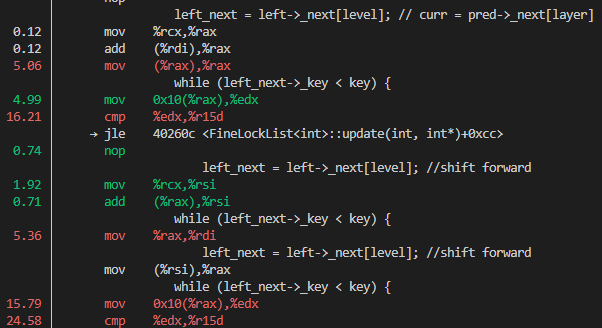
\includegraphics[width=3.4in]{ex1_s1_cycles.png} \\
\caption{perf record results for the fine-grained locking skip list on a 10,000,000 operations done on keys in a 200,000 range. Above is the cycle percentage across different functions and then a "zoomed in" line-by-line cycle breakdown for list search instructions found in the update() call.}
\end{figure}

Through observation of perf report, we find that the main time-consuming task for the lock-free skip list is the same as that of the coarse-grained skip list. Once again, list traversal takes up most of the cycles. The code pictured is nearly identical to that of before, down to the fact that the same instructions take most of the cycles. \\
Unlike the coarse-grained locking skip list, we also find that the fine-grained locks have much less of an effect on the overall cycle count as compared to the coarse-grained lock used previously. About 14\% of total cycles of the benchmark is used for pthread\_mutex\_lock and -unlock for the coarse-grained locking list, and only 7\% for the fine-grained locking list. This is expected because for the coarse-grained locking skip list, a mutex is locked and unlocked for every single operation, but for the fine-grained locking list, a mutex is only locked for update/removal operations. Furthermore, the coarse-grained locking skip list's lock is contended between every thread, but there are multiple, fine-grained locks that are not always grabbed by every thread. The cost of locking and unlocking is less if it can be stored in the cache and not contended between other threads. Thus, even though the fine-grained locking list takes more locks in the process of locking and unlocking, taking these locks is less expensive that doing so for the coarse-grained locking list. 

\textbf{Lock-free skip list:} 
\begin{figure}[h!]
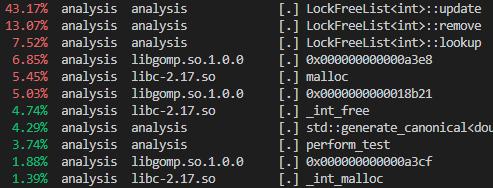
\includegraphics[width=3.4in]{ex1_s2_overall_cycles.png}
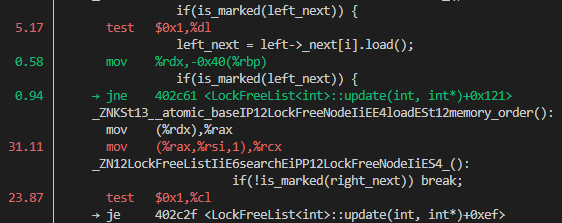
\includegraphics[width=3.4in]{ex1_s2_cycles.png} \\
\caption{perf record results for the lock-free skip list on 10,000,000 operations done on keys in a 200,000 range. Above is the cycle percentage across different functions and then a "zoomed in" line-by-line cycle breakdown for list search instructions found in the update() call.}
\end{figure}

For the lock-free skip list, it is less obvious that list traversal is the main operation of note, since the original code looks very different. (This is because the lock-free skip list's search function doubles as a function that removes a searched for node marked for deletion.) However, the cycle-heavy instructions continue to be the ones found in list search for both the update() and removal() functions, which dominate the overall cycle count percentage. 

Notice that unlike the other skip lists, the lock-free skip list uses atomic load operations for list traversal. This memory ordering constraint may have an impact on execution of these overall instructions. From the PSC benchmarks, we know that this atomic ordering doesn't have a cost significant enough to lower the performance of the lock-free list below that of the fine-grained locking case in all scenarios, but we know that the memory ordering constraint may impact the overall performance, since it affects the common-case instructions. However, as mentioned before, we have done some limited testing that found that choosing different memory orderings (by making use of C++ semantics) did not have an effect on performance. This is likely because memory ordering constraints govern how instructions can be reordered for execution; however, list traversal instructions involves highly dependent load and cmp instructions, which more several constrains reordering. 

%Generally, performance for our skip lists is memory-bound, and furthermore, it is largely memory bound due to poor locality of memory accesses in the concurrent skip list instead of additional memory accesses needed to manage.

%We also looked at the perf results on the PSC machines and found really interesting patterns. On PSC, due to factors from differences in architectures, we have a pretty small percentage of memory accesses actually dedicated to accessing skip list entries (around $25\%$). There's roughly $50\%$ spent on overhead and another $25\%$ for just accessing the input keys vectors. This emphasizes the importance of considering sequential implementations at lower numbers of threads, as this overhead could easily outweigh the benefits.
\pagebreak
\section{Additional Material}
Final recording: \href{https://www.youtube.com/watch?v=E-VfOaCNW-0}{15-618 Final Project: Concurrent Skip Lists} \\
Final Project repo: \href{https://github.com/gean2/parallel-cnn}{Public SkipList Repo} \\
Original repo: \href{https://github.com/gean2/skiplist-private}{skiplist-private}

\section{Contributions}
\begin{itemize}
    \item Initial research: Grace and Mckenna
    \item Coarse-grained locking and lock-free skip lists: Grace
    \item Fine-grained locking skip list: Mckenna (initial implementation) and Grace (debugging)
    \item Testing code: Grace
    \item Input distributions (uniform, normal, and bimodel) research and implementation: Mckenna
    \item Benchmarking: Mckenna (on GHC machines) and Grace (on PSC machines) 
    \item Performance analysis using perf: Grace
    \item Creating graphs: Mckenna
    \item Final report: Grace (Summary, Overview, Approach, PSC Performance Benchmarks, perf performance analysis), Mckenna (Background, Input distribution, GHC Performance Benchmarks)
    \item Final recording: Grace and Mckenna
\end{itemize}
We request credit be accorded 50/50.
\section{References}
\bibliographystyle{unsrt}
\bibliography{Bibliography}
\end{document}